
\chapter{Theory}
\label{chap:theo}
This section presents the theory as well as the whole individual steps in details of the implemented system. The implemented system or pose estimation pipeline as we refer interchangeably in this thesis is fed with two point clouds as input data, one generated from the CAD model and the other one is generated from the output sensory device(RealSense or Astra camera for purpose of comparison).

The 3D CAD model is rendered with the use of software tools described in the previous chapter. The pipeline has two parts, the first part as we refer as the offline stage where the CAD model is preprocessed, and the second one an online stage where the point cloud taken from the scence undergoes a preprocessing step similar to the one described above. In addition to, several filter techniques are used in order to segment the ROI (region of interest) and as a final step a matching stragy is applied where it outputs a 6-DOF pose estimation(ground truth) of the object.  

\section{Pose estimation pipeline}

Using a local feature base method, the pose estimation pipeline is seen in Figure \ref{fig:pipeline}. The pipeline used in this thesis is inspired in \cite{cadPipeline1}, \cite{cadPipeline2} and \cite{cadPipeline3}, with two major modifications, the first one is that the pipeline used in this thesis has the filtering part included in the preprocessing stage in order to better isolate the 3D object and the second modification is related to the matching strategy\cite{repMatching} where in most of the literatures, the preferred one is a hash table-based voting scheme, in contrast to the one used in this thesis, the hypothesize-and-test paradigm\cite{repMatching}, e.g. RANSAC scheme, which is suitable in this thesis. For more detail about matching strategies, the reader should refer to the reference. 


For the offline stage the 3D CAD model is rendered and it is converted to a point cloud data(PCD) format for a better subsequent use. As to the online stage, the pose estimation pipeline takes as input both clouds, the first one, a cloud from the 3D CAD model and the second one, a cloud from the scene, both clouds are filtered in order to remove noise and outliers. Since this is a tabletop application, we need to extract the candidate point cloud from the table. The table can be removed from the cloud with RANSAC as it was done in \cite{cadPipeline3}, which used to find the largest plane in the image. After, both clouds are downsampled by a Voxel Grid (VG) filtering method, and key points with their features descriptors are computed. Then the two clouds are feeding to the matching algorithm where a coerse 6-DoF pose (3 for translation and 3 for rotation) is obtained. The coerse pose is refined with an ICP algorithm registration. Each step is carefully explained in details ahead. 


\begin{figure}[!h]
\begin{center}
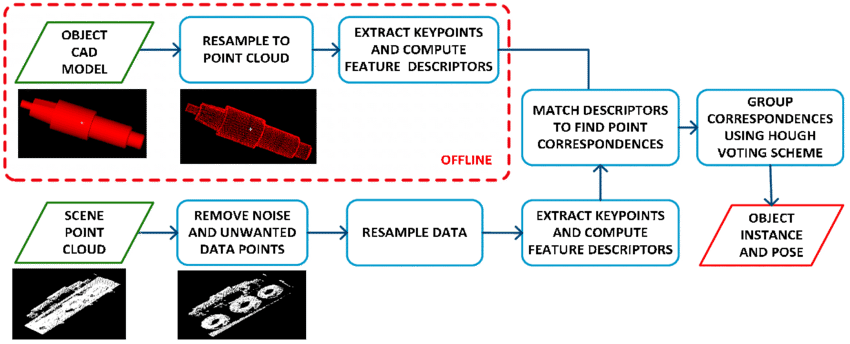
\includegraphics[width=3in]{figures03/pipeline.png}
\caption{General architecture of proposed pose estimation pipeline}%\cite{temp2}}
\label{fig:pipeline}
\end{center}
\end{figure}







\subsection{Preprocessing stage}

After the filtering step, which is only applied to the point cloud represented the scence. The two clouds are downsampled with technique already implemented in the Point Cloud Library, such as Voxelgrid (VG) filter or Approximate Voxelgrid filtering. This step is required for speed up the computation process. 
Since it is a computer vision problem known as Tabletop, it has a dominant plane. Therefore, RANSAC is used to find this dominat plane in the image. 

\subsection{Filtering a Point cloud}
The point cloud from the output sensory device contains undesired points, those are often noisy and contains outliers that lead to a high computation time and possibly produces a wrong pose estimation of object. Therefore, it is crucial to remove the noise and outliers from the point cloud in order to obtain accurate point clouds that are suitable for further processing. 

In order to identify these suitable point clouds, algorithms for filtering them are already implemented in the Point Cloud Library such as Conditional Removal, Radius/Statistical Outlier Removal, Color Filtering and Passthrough. 
Since there are few widely used techniques already developed for point cloud filtering. Some of them are aimed at reducing the amount of points in order to speed up the computation time. Others are used to discard outliars. In this thesis we exploit a simple and commonly used filtration pipeline which it has been proven to be an effective combination of methods in several works \cite{algFiltering}.

\subsubsection{Filtering a PointCloud using a PassThrough filter}
PassThrough passes points in a cloud based on constraints or threshold for one particular field (X,Y,Z) of the point type. Namely, it removes points where values of selected field are out of range. The filtration pipeline can be seen in the Figure \ref{fig:passthrough}. For more details and working examples the reader you should refer to \cite{pcl}

\begin{figure}[!h]
\begin{center}
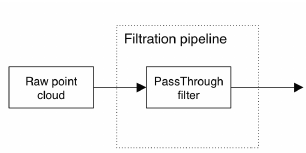
\includegraphics[width=3in]{figures03/passthrough.png}
\caption{Filtration pipeline used in this thesis}%\cite{temp2}}
\label{fig:passthrough}
\end{center}
\end{figure}
\subsubsection{Plane Segmentation}
Since the point cloud from the scene contains undesirable points such as points that represents a table where the object is kept. A further filtering is needed, such filtering is know as plane segmentation. And it is achievable with the RAMSAC based plane fitting method. RAMSAC method finds the largest set of points that fit to a plane. The plane equation in three dimensional point cloud can be defined as:

\begin{equation}
    ax+by+cz+d=0
\end{equation}
Where the a,b, and c are the parameters of the plane and d is the distance of the plane from the origin.

RAMSAC selects randomly three points from dataset and computes the parameters of the corresponding plane, after that it tries to enlarge the plane according to a given threshold,\cite{algPlane}. The step of segmenting the plane in order to remove it, is required condition for the subsequent use. Where a global registration is applied. 

\begin{algorithm}[H]
\SetAlgoLined
\KwResult{ o (object candidate point cloud) }
\KwData{p (3D point cloud), $\tau$ , MaxIter, IR }
 %initialization\;
 \While{$t<MaxIter$ - $InlierRatio>IR$}
 {
 Pick 3 points (A, B, C) at random from p \;
 Fit a plane (ax + by + cz + d = 0) to these 3 points\;
    AB = B - A\;
    AC = C - A\;
    N = AB x AC\;
    N has the values of (a, b, c)\;
    %d = −A^{T} \cdot N\\  
    Find outlier points o (object candidate points)\\
    %f(x)$>$\tau\\
    Here, f (x) is plugging in point x into the plane equation divided by the norm of N to measure residual and $\tau$ is the threshold\\
    Find Inlier Ratio as ratio of number of inlier points to total number of points
}
\caption{RANSAC for plane segmentation \cite{cadPipeline3}}
\end{algorithm}



\subsection{Extract geometric feature}
\subsubsection{3D keypoint Detection}

Keypoints are relevant points that maintain as much as possible the shape of the object. In order to identify these relevant points, detection methods are used. In addition to, keypoint are found by sampling the point cloud or downsampling the cloud with  VoxelGrid filter.

Voxel Grid filtering method \cite{algFiltering} creates a 3D Voxel Grid
(3D boxes in 3D space) for each one of the point cloud (model and scene cloud). Then, in each voxel, a point is chosen to approximate all the points that lie on that voxel. Usually, the centroid (an arithmetic mean) of these points or the center (the point in the interior that is equidistant from all points) of this voxel is used as the approximation. The centroid is slower than the center approximation. As a remark, the voxel grid method often drives to geometric information loss. See Figure \ref{fig:voxeldown} to see the result of applying voxel grid. For more information, the reader should see \cite{algDownsampling}


\begin{figure}[!h]
\begin{center}
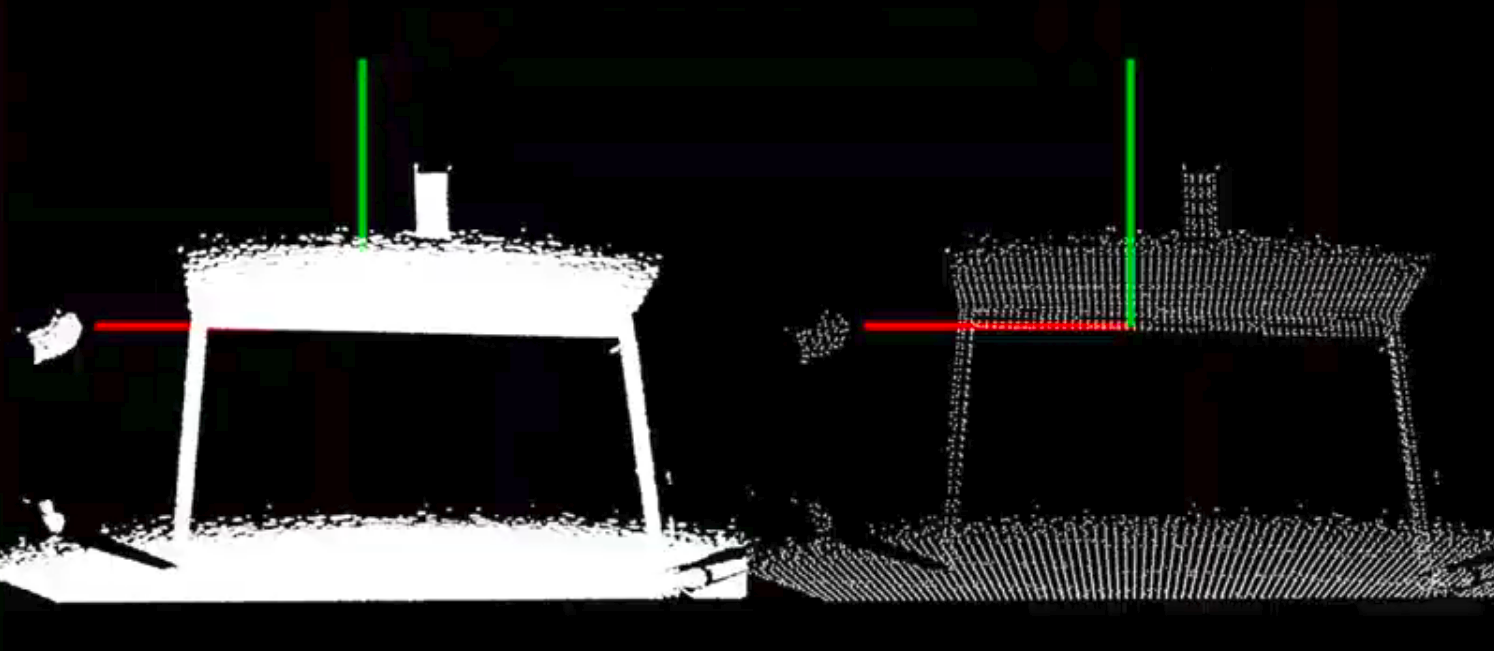
\includegraphics[width=3in]{figures03/voxelcloud1.png}
\caption{Left to Right: Input Image, Output after voxelGrid}%\cite{temp2}}
\label{fig:voxeldown}
\end{center}
\end{figure}


%\noindent
\textbf{Vertex normal estimation}

For the subsequent use, normal estimation of both point clouds, model and scene are computed. The approach implemented for computed the normal in this thesis is the vertex normal estimation, a directional vector associated with a vertex, intended as a replacement to the true geometric normal of the surface. The algorithm is already implemented in the open3D \cite{open3d} library. 
It computes the normal for every point by finding adjacent points and calculating the principal axis of the adjacent points.

\subsubsection{Local surface feature description}

Once the keypoints have been detected for the model and scene point clouds, geometric information of the local surface around those keypoints are extracted and encoded into feature descriptors. According to the approaches employed to construct the feature descriptors in \cite{survey}, classify into three group: signature based, histogram based and transform based method. In this thesis the approach of histogram based method is used. Namely, Fast Point Feature Histogram, FPFH, this method describe the local neighborhood of a s be generating histograms according to the geometric attributes(e.g.,normals) of the local surface.

\noindent
\textbf{Fast Point Feature Histogram}\\
Fast Point Feature Histogram (FPFH) in \cite{algFpfh}, is a developed version of the Point Feature Histogram (PFH) \cite{algFpfh} with a reduced computational complexity and same discriminative power. 

The generation of a FPFH descriptor consists of two steps. In the first step, a Darboux frame is defined $(u=n_{i},v=(p_{j} \times p_{i}) \cdot u,w=u\times v)$ for each point pair ($p_{i}$ and $p_{j}$). Then for each query point p it computes only the relationships between itself and its neighbors as follows:
\begin{align}
    \alpha& = v \cdot n_{j}\nonumber \\
    \phi&= \frac{u \cdot (p_{j} - p_{i})}{|p_{j} - p_{i}|}\label{pfheq} \\
    \theta &= \arctan(w \cdot n_{j} , u \cdot n_{i})\nonumber
\end{align}
The computation above is called a Simplified Point Feature Histogram (SPFH) which is binned by three angular variations ($\alpha , \phi , \theta$), then in the second step, the FPFH of each point is computed using both the SPFH of itself and the weighted ones of its neighbours as follow:

\begin{equation}\label{fpfheq}
    FPFH(p) = SPFH(p)+\frac{1}{k}\sum\limits_{n=1}^{k}\frac{1}{\omega _{k}}SPFH(p_{k})
\end{equation}

Where the weight $\omega _{k}$ represents the distance between query point p and a neighbor point $p_{k}$ in a given metric space.

\begin{figure}[!h]
\begin{center}
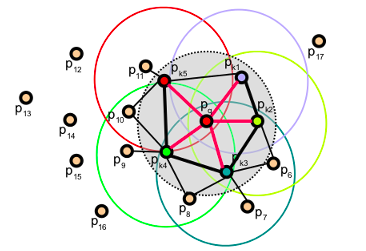
\includegraphics[width=3in]{figures03/fpfh1.png}
\caption{The influence region diagram for a Fast Point Feature Histogram. \cite{algFpfh}}.
\label{fig:fpfh}
\end{center}
\end{figure}

\subsection{Searching Strategies}

Once both point clouds (object and scene) have been filtered and their shape described, the next step is to find correspondences between them. Therefore, a searching strategy is needed in order to find the proper point correspondences between the two point clouds. Approaches vary in terms of how the correspondence between the scene and model feature is achieved, how a consistent set of matches is derived from the scene-model feature correspondence and how the pose is estimated from a consistent set of correspondence. In \cite{repMatching} describes the popular and important approaches to recognition and localization of 3D objects as follow: 
\begin{enumerate}
    \item hypothesize and test
    \item matching
    \item relational structures
    \item Hough(pose) clustering
    \item geometry hashing
    \item interpretation tree search and
    \item iterative model fitting techniques.
\end{enumerate}

In this thesis, a hypothesize-and-test approach is used. In the hypothesize-and-test paradigm, 3D transformation from the object model coordinate frame to the scene coordinate frame is first hypothesize to relate the model feature with the scene features. The transformation is used to verify the match of model features to the scene features. This hypothesized matching is either accepted or rejected depending on the amount of matching error, e.g.  RANdom SAmple and Consesus (RANSAC) is a representative method of this approach.

\subsubsection{RANSAC-based method} \label{sssec:num1}

RANdom SAmple and Consesus (RANSAC)\cite{repMatching} is an iterative method designed to find the parameters of a model from a set of data which contains outliers. Given an input noisy data, RANSAC finds the parameters that adjust the input data to a given model, discarding the outliers. In this thesis the RANSAC is used for global registration. In each RANSAC iteration, random points are picked from the model point cloud. Their corresponding points in the scene point cloud are detected by querying the nearest neighbor in the 33-dimensional FPFH feature space. A pruning step takes fast pruning algorithms to quickly reject false matches early. Only matches that pass the pruning step are used to compute a transformation, which is validated on the entire point cloud. 

\subsection{Local refinement}

The last step of the pipeline is the so-called refinement of the alignment achieved by a coarse matching generated in \ref{sssec:num1}. This step is also commonly referred to as "Fine matching". This alignment is further refined using a surface registration method, such as the Iterative Closest Point (ICP) algorithm, this method is a standard step after the initial estimates for the relative poses due to its robustness and reliability. 



\subsubsection{Iterative Closest Point}

The  key  concept  of  the  standard  ICP  algorithm  can  be summarized as follow:
\begin{enumerate}
    \item For each point in the source point cloud, find the closest point in the target point cloud.
    \item Estimate the combination of rotation and translation using a root mean square point to point distance metric minimization technique which will best align each source point to its correspondence found in the previous step. 
    \item Transform the source points using the obtained transformation.
    \item Iterate.
\end{enumerate}

Iteratively repeating these steps typically results in convergence to the desired transformation. In most implementations of ICP, the choice of the distance metric which we refer as $d_{max}$ represents a trade off between convergence and accuracy. A low value results in bad convergence(the algorithm becomes "short sighted"), a large value causes incorrect correspondences to pull the final alignment away from the correct value. The standard ICP algorithm is seen in Algorithm \ref{alg:algICP}. For more details about the ICP and its variants, the reader should refer \cite{repMatching} and \cite{algIcp}

Standard ICP is seen in Algorithm kkkk.

\begin{algorithm}[H]
\SetAlgoLined
\KwData{
\begin{enumerate}
\item Two point clouds: $A=\{a_{i}\}, B=\{b_{i}\}$
\item An initial transformation: $T_{0}$
\end{enumerate}
 }
\KwResult{The correct transformation, T, which aligns A and B}
 $T \leftarrow T_{0}$  \;
 \While{not converged}
 {
  \For{$i \leftarrow 1 \ \KwTo \ N$}{
   $m_{i} \leftarrow FindClosestPointInA(T \cdot b_{i})$\;
   %-----------
    \eIf{$\|m_{i}-T \cdot b_{i}\| \leqslant d_{max}$}{
    $ \omega _{i} \leftarrow 1$\;
    }{
    $ \omega _{i} \leftarrow 0$\;
	}
  }
  %--------------
   $T \leftarrow \underset{T}{\mathrm{argmin}} {\sum \limits_{n=1}^{N}\omega _{i}\|m_{i}-T \cdot b_{i}\|^{2}}$\;
}
\caption{Standar ICP}
\label{alg:algICP}
\end{algorithm}




































